\normaltrue
\correctionfalse

%\UPSTIidClasse{12} % 11 sup, 12 spé
%\newcommand{\UPSTIidClasse}{12}

\exer{Banc d'épreuve hydraulique $\star$ \label{C2:091D:63}}
\setcounter{question}{0}\UPSTIcompetence[2]{C2-09}
\index{Compétence C2-09}
\index{Principe fondamental de la dynamique}
\index{PFD}
%\index{Mécanisme à 1 rotation}
\index{Banc d'épreuve hydraulique} % CCP PSI 2010
\ifcorrection
\else
\marginnote{\textbf{Pas de corrigé pour cet exercice.}}
\fi

\ifprof
\else
Un schéma cinématique simplifié du chariot arrière, ainsi que les grandeurs cinématiques et cinétiques,
sont donnés figure suivante.
La chaîne de puissance comporte un moteur hydraulique, un réducteur roue et vis sans fin, un réducteur à
engrenages parallèles et un système pignon-crémaillère.
Le guidage du chariot est modélisé par une glissière.



\begin{figure}[H]
\centering
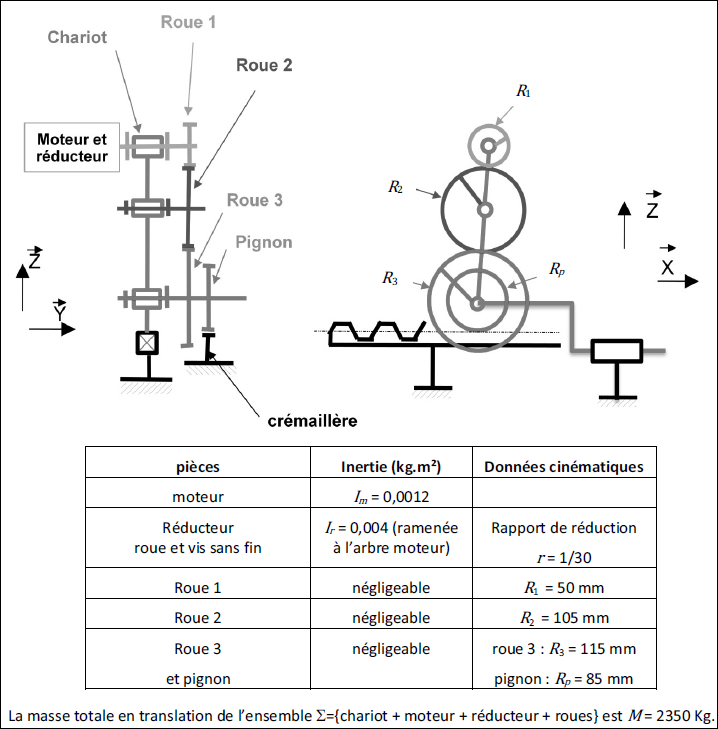
\includegraphics[width=\linewidth]{63_01}
%\caption{\label{61_01} Loi de commande de vitesse en trapèze}
\end{figure}


On note $C_m$  le couple moteur, $\omega_m$ sa vitesse de rotation par rapport au bâti, et $V$ la vitesse du chariot.
La loi de vitesse du chariot pendant la totalité du trajet est présentée ci-dessous.

\begin{figure}[H]
\centering
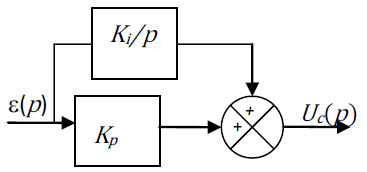
\includegraphics[width=\linewidth]{63_02}
%\caption{\label{61_01} Loi de commande de vitesse en trapèze}
\end{figure}


\begin{itemize}
\item On note $t_r$ la durée de la phase de déplacement rapide, $t_l$ la durée de la phase lente, $t_f$ la durée
totale, $t_a$ la durée de la phase d'accélération. Chacune des 2 phases de décélération dure $t_a/2$.
\item La course pendant la phase de déplacement en vitesse rapide (de 0 à $t_r$) est au maximum de
$c_{rap}= \SI{6,24}{m}$ (pour le tube le plus court que peut tester le banc) et pendant la phase en vitesse
lente (de $t_r$ à $t_f$) $c_{\text{lent}}= \SI{1,56}{m}$.
\item La durée maximale du déplacement total (phase rapide + phase lente) est limitée à \SI{20}{s}.
\item La vitesse du chariot, lors de la phase rapide, $V_{\text{rap}}$ est limitée à \SI{0,5}{m/s}.
\item On considérera que le module de l'accélération $a$ du chariot est identique pendant toutes les
phases d'accélération et de décélération.
\end{itemize}

\fi

\question{Exprimer $c_{\text{lent}}$ et $c_{\text{rap}}$ en fonction de $t_a$, $t_l$ et $t_r$.}
\ifprof
\else
\fi

\question{En déduire les valeurs numériques de $t_r$ et de $t_a$. En déduire l'accélération $a$ du chariot.}
\ifprof
\else
\fi

\question{Déterminer $\omega_m$ en fonction de $V$ et des données cinémtiques utiles.}
\ifprof
\else
\fi

\question{En déduire les valeurs numériques de la vitesse maximale du moteur $\omega_m$ et de l'accélération angulaire $\dot{\omega}_m$ pendant les phases d'accélération et de décélération.}
\ifprof
\else
\fi

\question{Donner l'expression de l'énergie cinétique de l'ensemble $\Sigma$ par rapport au référentiel galiléen bâti.}
\ifprof
\else
\fi

\question{En déduire l'expression de l'inertie équivalente de cet ensemble ramenée à l'axe de sortie du
moteur, notée $J_{\text{eq}}$ en fonction de $M$, $I_m$, $I_r$ et des données cinématiques utiles. Application
numérique.}
\ifprof
\else
\fi


\ifprof
\else
\begin{itemize}
\item Les efforts résistants sur le chariot sont modélisés par un glisseur $F$ d'amplitude \SI{500}{N}.
\item Le rendement de l'ensemble du mécanisme (réducteur roue et vis sans fin, réducteur à axes parallèles) est $\eta= 0,3$.
\item On prendra une accélération angulaire maximale du moteur $\dot{\omega}_m$ égale à \SI{250}{rad.s^{-2}} et une inertie totale équivalente ramenée à l'arbre moteur $J_{\text{eq}}$ égale à \SI{0,01}{kg.m^2}.
\end{itemize}
On se propose de déterminer le couple nécessaire du moteur.
\fi

\question{Déterminer l'expresion du couple $C_m$ à fournir par le moteur en fonction de $\dot{\omega}_m$, $J_{\text{eq}}$ et $F$. Calculer $C_m$.}
\ifprof
\else
\fi



\ifprof

\else
\ifcolle
\else
\footnotesize
\begin{enumerate}
 \item $c_{\text{lent}}=\dfrac{V_{\text{rap}}}{2}t_l$ et $c_{\text{rap}}=V_{\text{rap}}\left(t_r - \dfrac{1}{2}t_a\right)$.
 \item $t_a=\SI{2,56}{s}$, $t_l=\SI{6,24}{s}$, $t_r=\SI{13,76}{s}$ et $a =\SI{0,19}{m.s^{-2}}$. 
 \item $\omega_M = - \dfrac{VR_3}{rR_1R_p}$.
 \item $\omega_m = -\SI{406}{rad.s^{-1}}$ et  $\dot{\omega}_m= -\SI{158}{rad.s^{-2}}$.
 \item $\ec{\Sigma}{0} = \dfrac{1}{2}MV^2 + \dfrac{1}{2}\left( I_M + I_r \right)\omega_m^2$.
 \item $J_{\text{eq}} = I_M + I_r + M \left( \dfrac{rR_1 R_p}{R_3}\right)^2 = \SI{0,00877}{kg.m^2}$.
 \item $C_M \dfrac{J_{\text{eq}} \dot{\omega}_m + F \dfrac{rR_1R_p}{R_3}}{\eta} = \SI{10,4}{Nm}$ (rendement à voir...).
\end{enumerate}
\fi

\normalsize

\begin{flushright}
\footnotesize{Corrigé  voir \ref{C2:091D:63}.}
\end{flushright}%
\fi